\def\notedate{2023.02.01}
\def\currentauthor{Журавлев Н.В. (РК6-72Б)}
\notestatement{rndhpcedt}{Алгоритм обхода графа (возможно переименовать в описание алгоритма и название записки)}

\begin{task}
Дано: Ориентированный граф с возможным наличием циклов.
Необходимо: разработать алгоритм обхода графа
\end{task}

Основная идея заключается в том, чтобы программы двигалась по графу как человек. Алгоритм двигается к следующей возможной вершине, если она одна, но если их две, то выбирает случайную (на данном шаге возможно добавление эвристики), а остальные заносит в специально созданный стек, за исключением случаев, когда селектор разрешает только одно перемещение, затем выполняется переход. Если в вершине, в которую перешли, требуется более одной дуги для продолжения, то алгоритм в данной вершине делает пометку, что одна дуга уже пришла, затем берёт вершину из стека и продолжает обход относительно неё. При возвращении в эту же вершину, если достаточно вершин пришло, то уже проходит через неё. И данный процесс происходит пока не дойдёт до конечной точки графа.

Чтобы реализовать данный алгоритм необходимо сделать класс дуги и в класс узла добавить поля, которые определяют необходимое число для перехода через данный узел и количество дуг, которые уже пришли в узел. Класс дуги содержит два поля: начальный узел и конечный узел. 

Рассмотрим работу алгоритма на примере графа представленный на рисунке \ref{fig:graph}. Начальная вершина называется "Start", а конечная "End". Селекторы в данном примере отсутствуют, однако их добавление не помешает корректной работе алгоритма.

\begin{figure}[h]
    \centering
    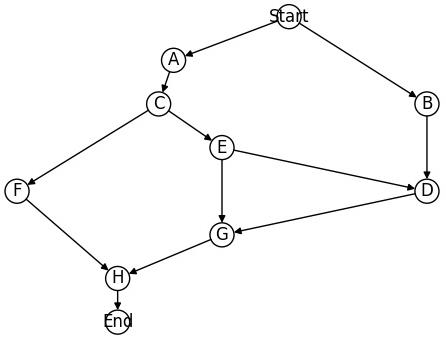
\includegraphics[width=0.6\linewidth]{ResearchNotes/rndhpc_alg_edt_2023_02_01/graph.jpg}
    \caption{Рассматриваемый граф}
    \label{fig:graph}
\end{figure} 

Так как из точки "Start" идёт две дуги, то выбираем случайную из них, допустим это будет дуга в вершину "A", совершаем переход в неё, а вершина "B" заносится в стек. Затем из-за того, что всего доступна только 1 вершина, переход идёт в вершину "C".

После этого опять происходит ситуация, что из вершины идёт две дуги. Поступаем аналогично и выбираем вершину "E", заносим в стек вершину "F". Затем по аналогичной ситуации переходим из "E" в "D", а "G" заносим в стек.

В случае перехода в вершину "D", она требует две дуги, поэтому достаём из стека вершину и это вершина "G", которая тоже требует две дуги, поэтому снова достаём из стека вершину. Этой вершиной является "F", затем переходим в неё, и далее в вершину "H", которая требует 2 дуги.

Снова достаём из стека вершину и это вершина "B" из неё идёт в вершину "D", т.к. уже одна дуга уже пришла, то из неё можно перейти в вершину "G". Из которой тоже можно перейти по таким же причинам, затем аналогично "H", после этого переходим в "End" и работа алгоритма заканчивается.

\noteattributes{}